This section presents a systematic mapping analysis. The aim of our
bibliographic study using the systematic mapping methodology
\cite{Petersen:2008} is to (i) categorize and quantify the key contributions and
the evolution of the research done on big data, MapReduce design patterns and
its classifications; and (ii) discover open issues and limitations of existing works.
The results of the systematic mapping are presented as
bubble plots. These visual representations have two main
benefits: (i) it can show the relevance of the mapping facets/categories
has changed over time and (ii) it can reveal research opportunities
hidden on the blanks found among classification categories, pointing
topic areas and types of publications yet to be investigated. Our study is guided
by three research questions:

\begin{itemize}
\item {\em RQ1: Which are the main MapReduce design patterns used in data
analysis?} This question is devoted to measure the map reduce design patterns
used in big data analysis and to verify which of them are the most common.

\item {\em RQ2: What type of solutions have been proposed considering MapReduce
design patterns?} This question will help us to identify how map reduce design patterns are used in data analysis, and also
what type of solution have been proposed for each kind of pattern or
composition of patterns. It will let us identify how the patterns can be
composed to a better big data analysis result.
 
\item  {\em RQ3: Which type of relationship between patterns are proposed to
improve the results of big data analysis?} The map reduce design patterns are
classified considering and addressing different aspects
according big data domain. There is a list o patterns organized into categories
such as summarization, filtering, data organization and join patterns. These
patterns can be composed in order to get a better result of the big data
analysis. Thus, this research question aims to verify if the patterns are often
compounds, and which kind of composition is made.
\end{itemize} 

% %.........................................................
% \subsection{Search and Retrieval of Papers}
% 
% %\subsection{Expressing the  query for generating a data collection}
% %.........................................................
% Considering the research questions, we defined a set of keywords to be used for
% searching relevant works. Based on these keywords and their
% correlated words the query used was:        
%  
% \begin{quote} \sl
% \qquad  (big data \textbf{OR} bigdata \textbf{OR} map reduce \textbf{OR}
% map-reduce \textbf{OR} mapreduce \textbf{OR} hadoop \textbf{OR} pig)
% 
% \textbf{AND}
% 
% \qquad (design patterns \textbf{OR} designpatterns \textbf{OR}
% design-patterns \textbf{OR} design pattern
% \textbf{OR} designpattern \textbf{OR} design-pattern)
% \end{quote}

% 
% \begin{table}\centering
% \begin{tabular}{|l|c|c|c|} \hline
% \textbf{Source/Action}	& \textbf{Included}	& \textbf{Excluded}	& \textbf{Total}	\\ \hline
% \textit{ACM-DL}				& 3								& 3								& 6						\\ \hline
% \textit{IEEE}						& 28								& 156								& 188					\\ \hline
% \textit{Science Direct}	& 1								& 1							& 2					\\ \hline
% \textbf{Total}					& \textbf{32}			& \textbf{164}			& \textbf{196}	\\ \hline
% \end{tabular}
% \caption{\label{table:Sources}Sources and number of papers.}
% \end{table}

We searched and filtered relevant works in four steps. 
In the first  step we
searched in four databases: \textit{Science Direct}\footnote{\tt
http://www.sciencedirect.com/}, \textit{IEEE}\footnote{\tt
http://ieeexplore.ieee.org/} and \textit{ACM Digital Library}\footnote{\tt
http://dl.acm.org/}. %(see table \ref{table:Sources})
We retrieved 196 works. 
The search was done for relevant publications from 1998 to 2014. 
We stored in several spreadsheets (one per database) the title, year,  and abstract of each reference we found. 

In the second step, we perform a data cleaning by excluding repeated works.  

We performed another filtering procedure by screening the title and the abstract
of the papers, looking for those papers that are relevant to our study.
In this process, we excluded 164 works. 
% The columns \textbf{Included} and \textbf{Excluded} in Table~\ref{table:Sources}
% show the number of papers that were considered (resp. excluded) on our study.
 
Finally, in the last step we built the final data collection using exclusion
and inclusion criteria shown in table \ref{table:criteria}. The final data
collection contained 32 papers.

\begin{table}\centering \small
\begin{tabular}{|l|} \hline
\textbf{Inclusion criteria}		\\ \hline\hline
- Text in English								\\ \hline
- Peer reviewed journals, conferences or workshops	\\ \hline
- PhD and master thesis	\\ \hline
- Focus on Map Reduce Design Patter and Big Data				\\ \hline\hline
\textbf{Exclusion criteria}		\\ \hline\hline
- Abstracts, tutorials, short papers, PhD workshops, demonstrations, technical reports		\\ \hline
- Papers dealing with service service lookup		\\ \hline
- Papers dealing with service matching 	\\ \hline
\end{tabular}
\caption{\label{table:criteria} Inclusion and exclusion criteria.}
\end{table}

%\subsection{Dimensional Analysis} 

According to our research questions and to our interests, the papers were
classified into four analysis facets.
Analysis facets are classification schemes  that define mapping categories to cluster and analyze the papers. 
All 32 papers in our mapping were analyzed to discover their contribution to
each of the facets defined for our study.
The result of this process is a classification of papers for the dimensions of each facet.

The relevant frequent terms in the papers retrieved can be considered as
dimensions that represent subcategories within the facets that group them. Next
we present the facets and demensions we defined for the classification scheme: 
  
\begin{enumerate}
\item \textbf{\textit{Patterns Classification:}} This facet groups the
dimensions \textit{Summarization, Filtering, Data Organization, Join} and \textit{Input/Output}.

\item \textbf{\textit{Application Domain:}} This facet groups the dimensions
\textit{Graph, Data Warehouse, Standard Big Data} and \textit{Network}.

\item \textbf{\textit{Research Type:}} This facet groups the dimensions
\textit{Proposed Solution, Evaluation, Validation} and \textit{Opinion}.

\item \textbf{\textit{Contribution:}} This facet groups the dimensions
\textit{Algorithm, Model, Tool, Literature Analysis, Mathod} and \textit{New Pattern}.

\end{enumerate}
 
\subsection{Quantitative Analysis}

Considering the mapping processes presented above, this
section discusses the quantitative analysis that we propose as a result of
applying the Systematic Mapping methodology.  

In order to observe the evolution of the publication trends we analyse the
results from the time screen between the years 2010 and 2014 (see Figure
\ref{fig:contribution-per-year}). It was from 2010 which the first works
concerning MapReduce design patterns started to be published.         

The following lines discuss the answers. We combined the facets for answering
the research questions proposed for guiding our study. 

\bigskip
\textbf{\textit{RQ1: Which are the main MapReduce design patterns used in data
analysis?}} 
    
The facets Application Domain, Research Type and Pattern Classification give
elements for determining which patterns have been used in data analysis (Figures
\ref{fig:research-patterns-domain}). 
% and \ref{fig:patterns-domain}).

The resulting shows (in Figure \ref{fig:research-patterns-domain}, right side)
that most reserches type present \textit{Proposed Solution} and
\textit{Evaluation} of the application of the patterns, 17 (53.12\%) and 13
(40.62\%) papers, respectively. \textit{Validation} propositions are 12.5\% of
the works with 4 papers, and there is work that considers \textit{Opinion}
research type. This results considers the relation between the Research Type
facet and the Pattern Classification facet. From those, and considering the
classification proposed by \cite{White:2012}, the design patterns most used are
the \textit{I/O} and \textit{Join} patterns, with 8 (25.00\%) and 6 (18.75\%)
papers, respectively.  The Filtering, Data Organization and Summarization
patterns appers in 4 (12.50\%), 3 (9.38\%) and 2 (6.25\%) works,
respectively. 11 paper (34.38\%) of the papers consider othe classification of
design patterns for MapReduce, some of then presented in \cite{pig-designpattern:2014}.
 
For the Domain Application and Research Type relation (in Figure
\ref{fig:research-patterns-domain}, left side), the Standard Big Data domain is
that one which most appers with 28 papers (87.50\%). Graph domain comes just
after with 10 (31.25\%) works, and then Network and Data Warehouse with 4
(12.5\%) and 2 (6.25\%) papers, respectively.  

\begin{figure}[hbtp]
\centering
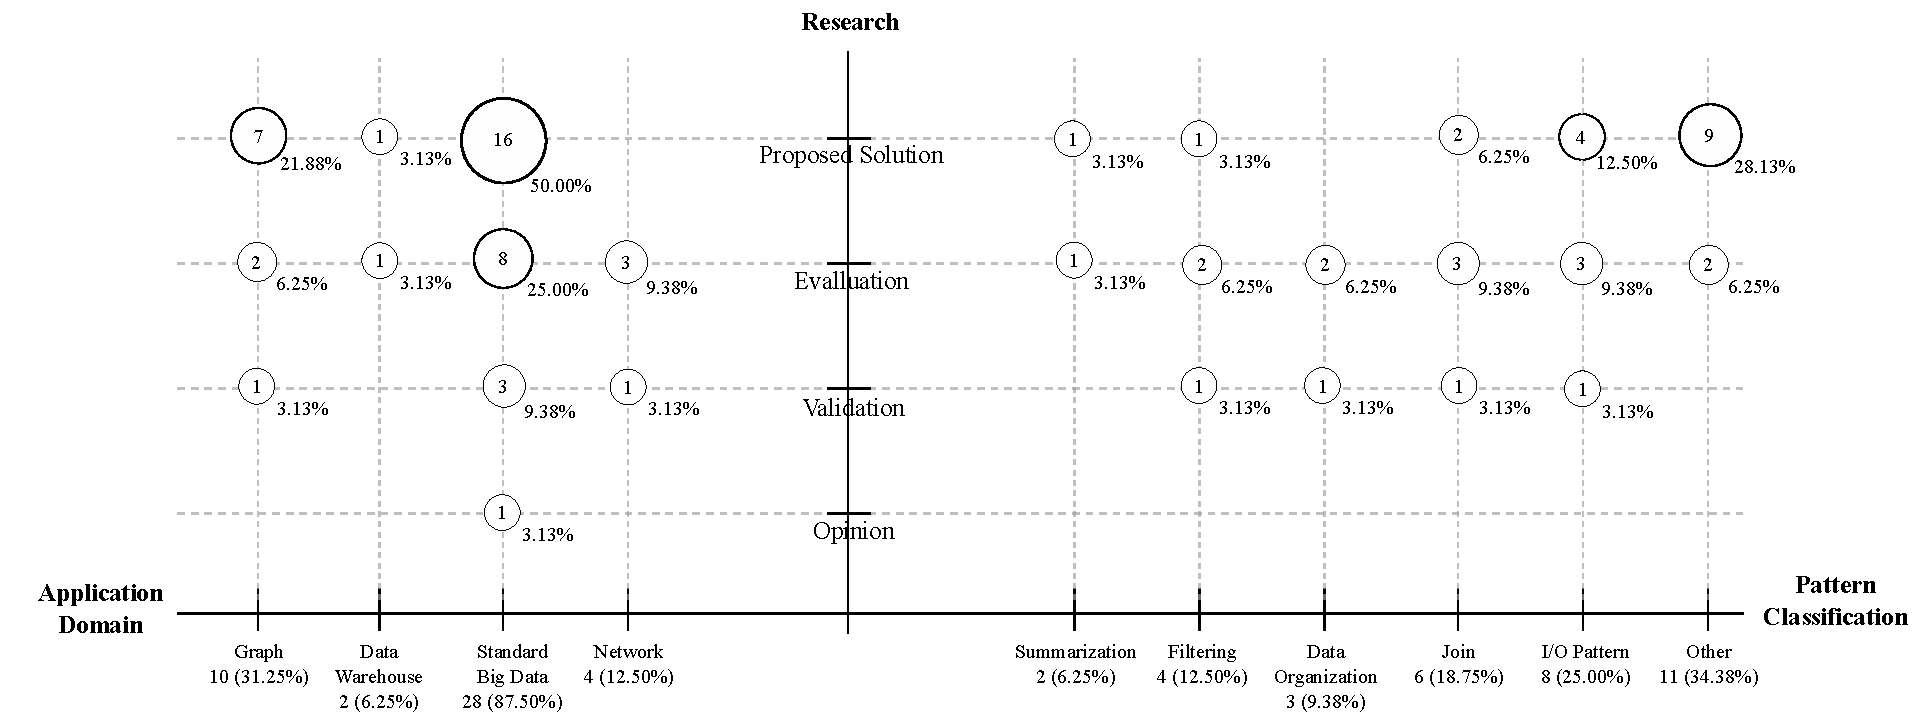
\includegraphics[width=0.99\textwidth]{figs/Research-Patterns-Domain.pdf}
\caption{Facet Research being related with the facets Pattern
Classification and Application Domain}
\label{fig:research-patterns-domain}
\end{figure}

% \begin{figure}[hbtp]
% \centering
% 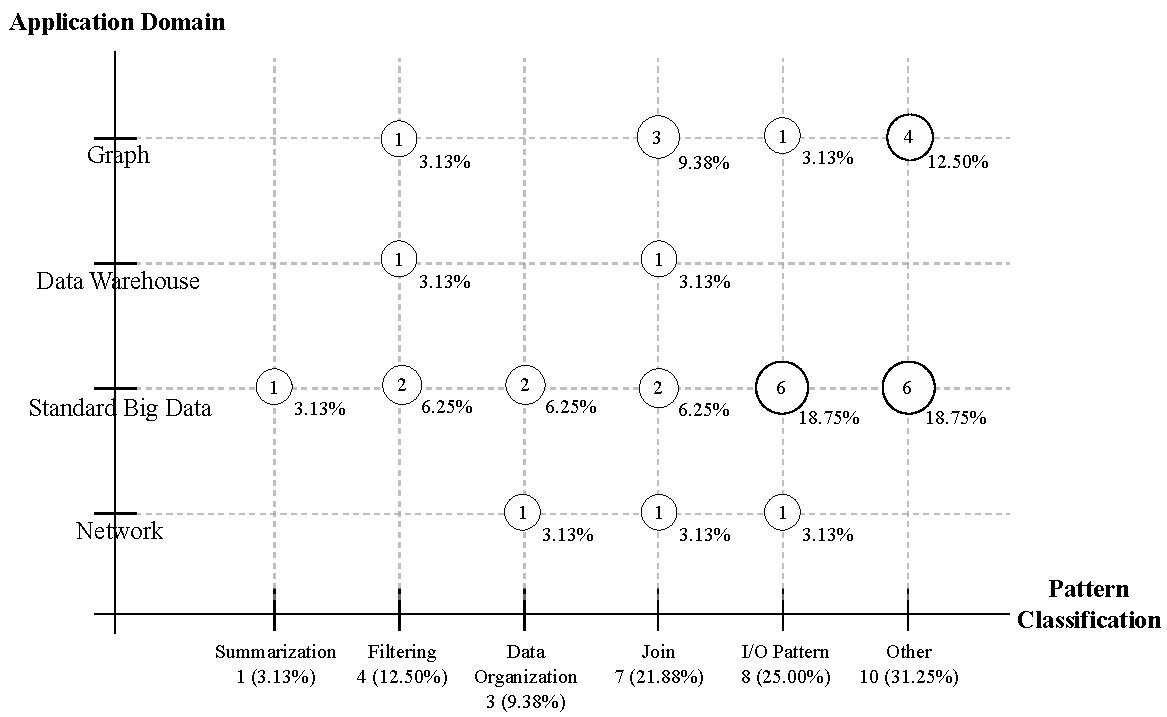
\includegraphics[width=0.79\textwidth]{figs/Patterns-Domain.pdf}
% \caption{Facets Pattern
% Classification and Application Domain}
% \label{fig:patterns-domain}
% \end{figure}
  
\bigskip
\textbf{\textit{RQ2: What type of solutions have been proposed considering
MapReduce design patterns?}}

The facet Contribution related with the facets Research Type and Pattern
Classification give elements for determining which type of solutions been
proposed for MapReduce design patterns (Figure
\ref{fig:contribution-patterns-domain}).

The solution most proposed considering the Application domain (felt side of
Figure \ref{fig:contribution-patterns-domain}) is Algorithms, Method and Tools
for big data analysis, considering MapReduce design patterns. The two types of
contribution represents 13 (40.63\%), 9 (28.12\%) and 9 (28.12\%) papers,
respectively. Literature Analysis and Model have the same number of
contributions, 7 (21.87\%) papers. Only 4 (12.50\%) works propose new patterns,
different from those already classified
\cite{White:2012,pig-designpattern:2014}. Considering all types of contribution,
the Standard Big Data analysis is the domain that are most applied, 29
(90.63\%). Ghaph domain has 13 (40.63\%) works which propose a solution using
some of the design patterns.

For the right side relation of Figure \ref{fig:contribution-patterns-domain},
Contribution and Pattern Classification, the result is similar from that of
\textit{RQ1}. textit{I/O} and \textit{Join} patterns, both with 8 (25.00\%)
papers, are the patterns that most appears in solutions for MapReduce design
patterns. The most frequantly type of contribution is also \textit{Algorithm}
and \textit{Tool}.

\begin{figure}[hbtp]
\centering
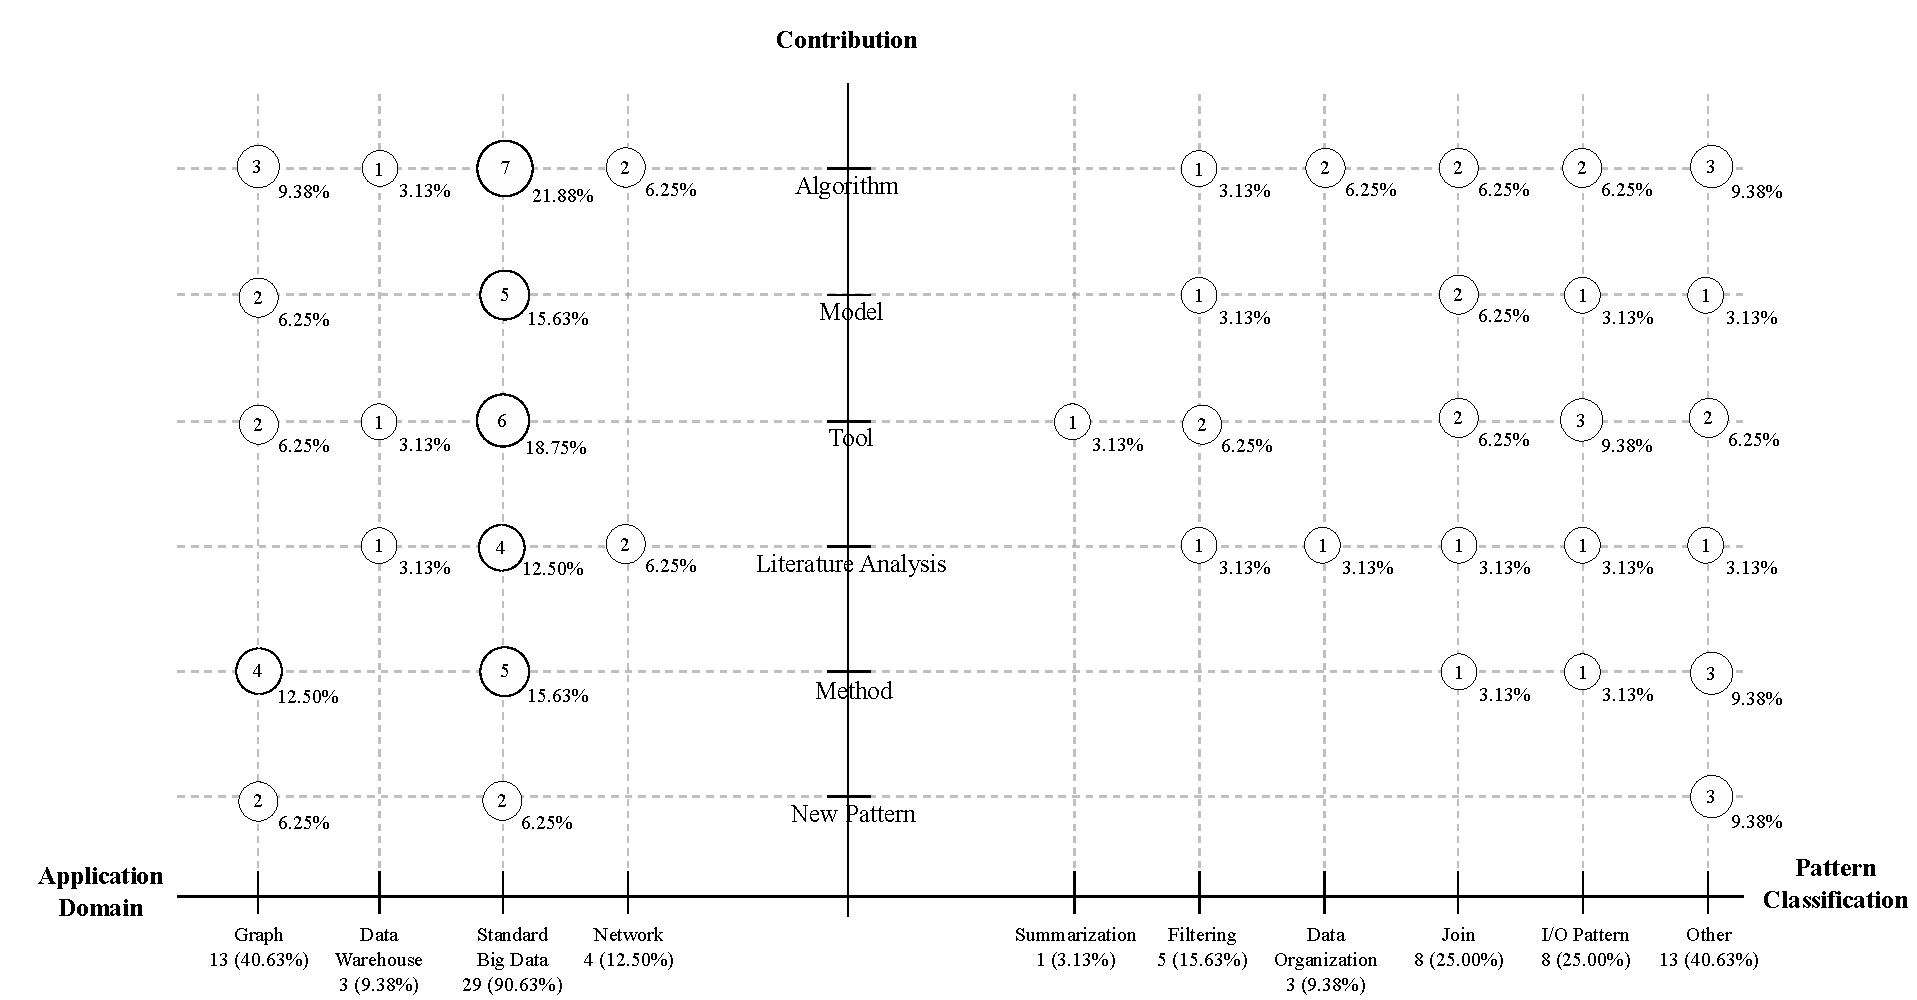
\includegraphics[width=0.99\textwidth]{figs/Contribution-Patterns-Domain.pdf}
\caption{Facet Contribution being related with the facets Pattern
Classification and Application Domain}
\label{fig:contribution-patterns-domain}
\end{figure}

\bigskip
\textbf{\textit{RQ3: Which type of relationship between patterns are proposed to
improve the results of big data analysis?}}
 
Considering the papers that were included in the analysis from the criterias,
there was no specificy reference for the apply composition or relationship
between patterns to improve the results of big data analysis. 


As the use of MapReduce design patterns is relatively new, the
composition of different types of patterns should be one factor by which
there are no reference works that considers this topic.
Thus we see a challenge and a gap to be considered for improving data analysis
fromo composition or  relationship between patterns with the goal of finding
improved results in the analysis.
 
What we can see is the evolution between the years 2010 and 2014 (Figure
\ref{fig:contribution-per-year}), with the increase of publications considered the use of design patterns to analyze
mapreduce for big data. As the first classification of patterns using Hadoop
apperead only in 2012, and the classification of patterns for Pig appeared
in 2014, this may be another factor to be considered to not find references
which goal the relationship between existing patterns.
  
\begin{figure}[hbtp]
\centering
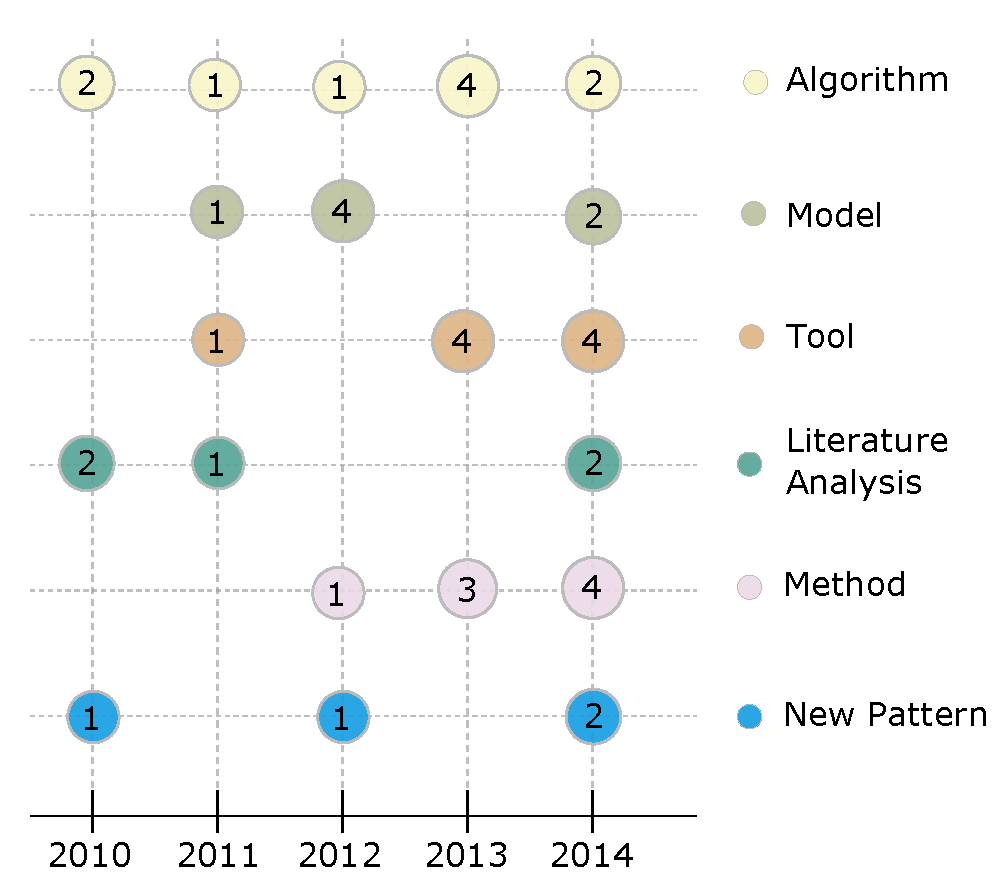
\includegraphics[width=0.69\textwidth]{figs/ContributionPerYear.pdf}
\caption{Contribution per year}
\label{fig:contribution-per-year}
\end{figure}

From 2010 to 2014 the number of paper grew up from 5 to 16. The type of
contribution most considered wwere the proposal of new Algorithm and Tool
(Figure \ref{fig:contribution-per-year}). However, the number of proposed
solutions for num Method, New Patterns and Literature Analysis were the ones
which grew up from 2013 and 2014. 

According to our quantitative analysis we observe that the definition of new
patterns, or a new classification has started to be considered for big data
analysis. 

%%%%%%%%%%%% FINALIZAR SECAO %%%%%%%%%%%%  



% %_____________________________________________________
% \paragraph{\bf\em Contribution} 
% %_____________________________________________________
% Refers to the concrete result described in a reference: {\em algorithm},	{\em
% model}, 	{\em tool}, {\em literature analysis}, and {\em	method}.
% \begin{table}\centering
% \footnotesize
% \begin{tabular}{|c|c|}\hline
% \textbf{Dimension} & \textbf{References} \\ \hline
% %\multirow{6}{*}{\begin{sideways} \textbf{Sw Pr Phase} \end{sideways} } & 
% %\\ \cline{2-3}
% Algorithm	& 
% \parbox{0.6\textwidth}{\cite{}.}
% \\ \hline
% Model	& 
% \parbox{0.6\textwidth}{\cite{}.}
% \\ \hline
% Tool		&
% \parbox{0.6\textwidth}{\cite{}.}
% \\ \hline
% Literature Analysis		&
% \parbox{0.6\textwidth}{\cite{}.}
% \\ \hline
% Method	&	
% \parbox{0.6\textwidth}{\cite{}.}
% \\ \hline
% 
% \end{tabular}
% \caption{\label{table:biblioContrib} Facet: Contribution.}
% \end{table}
% 
% %_____________________________________________________
% \paragraph{\bf\em Research Type} 
% %_____________________________________________________
% Refers to the concrete result described in a reference: {\em proposed solution},
% {\em evaluation}, 	{\em validation}, and {\em opinion}.
% \begin{table}\centering
% \footnotesize
% \begin{tabular}{|c|c|}\hline
% \textbf{Dimension} & \textbf{References} \\ \hline
% %\multirow{6}{*}{\begin{sideways} \textbf{Sw Pr Phase} \end{sideways} } & 
% %\\ \cline{2-3}
% Proposed Solution	& 
% \parbox{0.6\textwidth}{\cite{}.}
% \\ \hline
% Evaluation	& 
% \parbox{0.6\textwidth}{\cite{}.}
% \\ \hline
% Validation		&
% \parbox{0.6\textwidth}{\cite{}.}
% \\ \hline
% Opinion		&
% \parbox{0.6\textwidth}{\cite{}.}
% \\ \hline
% \end{tabular}
% \caption{\label{table:biblioResearch} Facet: Research Type.}
% \end{table}
% 
% 
% %_____________________________________________________
% \paragraph{\bf\em Pattern Classification} 
% %_____________________________________________________
% Refers to the concrete result described in a reference: {\em summarization},
% {\em filtering}, 	{\em data organization}, {\em join}, 	{\em metapattern}, 
% {\em i\/o pattern}, and {\em other}.
% \begin{table}\centering
% \footnotesize
% \begin{tabular}{|c|c|}\hline
% \textbf{Dimension} & \textbf{References} \\ \hline
% %\multirow{6}{*}{\begin{sideways} \textbf{Sw Pr Phase} \end{sideways} } & 
% %\\ \cline{2-3}
% Summarization	& 
% \parbox{0.6\textwidth}{\cite{}.}
% \\ \hline
% Filtering	& 
% \parbox{0.6\textwidth}{\cite{}.}
% \\ \hline
% Data Organization		&
% \parbox{0.6\textwidth}{\cite{}.}
% \\ \hline
% Join		&
% \parbox{0.6\textwidth}{\cite{}.}
% \\ \hline
% Metapattern		&
% \parbox{0.6\textwidth}{\cite{}.}
% \\ \hline
% I\/O Pattern		&
% \parbox{0.6\textwidth}{\cite{}.}
% \\ \hline
% Other		&
% \parbox{0.6\textwidth}{\cite{}.}
% \\ \hline
% \end{tabular}
% \caption{\label{table:biblioResearch} Facet: Research Type.}
% \end{table}
% 
% %_____________________________________________________
% \paragraph{\bf\em Application Domain} 
% %_____________________________________________________
% Refers to the concrete result described in a reference: {\em graphs},
% {\em data warehouse}, 	{\em standard big data}, and {\em network}.
% \begin{table}\centering
% \footnotesize
% \begin{tabular}{|c|c|}\hline
% \textbf{Dimension} & \textbf{References} \\ \hline
% %\multirow{6}{*}{\begin{sideways} \textbf{Sw Pr Phase} \end{sideways} } & 
% %\\ \cline{2-3}
% Graphs	& 
% \parbox{0.6\textwidth}{\cite{}.}
% \\ \hline
% Data Warehouse	& 
% \parbox{0.6\textwidth}{\cite{}.}
% \\ \hline
% Standard Big Data 		&
% \parbox{0.6\textwidth}{\cite{}.}
% \\ \hline
% Network		&
% \parbox{0.6\textwidth}{\cite{}.}
% \\ \hline
% \end{tabular}
% \caption{\label{table:biblioResearch} Facet: Research Type.}
% \end{table}

% %_____________________________________________________
% \paragraph{\bf\em Usage Standard}  
% %_____________________________________________________
% Refers to the concrete result described in a reference: {\em single pattern},
% and {\em composed pattern}.
% \begin{table}\centering
% \footnotesize
% \begin{tabular}{|c|c|}\hline
% \textbf{Dimension} & \textbf{References} \\ \hline
% %\multirow{6}{*}{\begin{sideways} \textbf{Sw Pr Phase} \end{sideways} } & 
% %\\ \cline{2-3}
% Single Pattern	& 
% \parbox{0.6\textwidth}{\cite{}.}
% \\ \hline
% Composed Pattern	& 
% \parbox{0.6\textwidth}{\cite{}.}
% \\ \hline
% \end{tabular}
% \caption{\label{table:biblioResearch} Facet: Research Type.}
% \end{table}
 
    
% \begin{figure}[hbtp]
% \centering
% 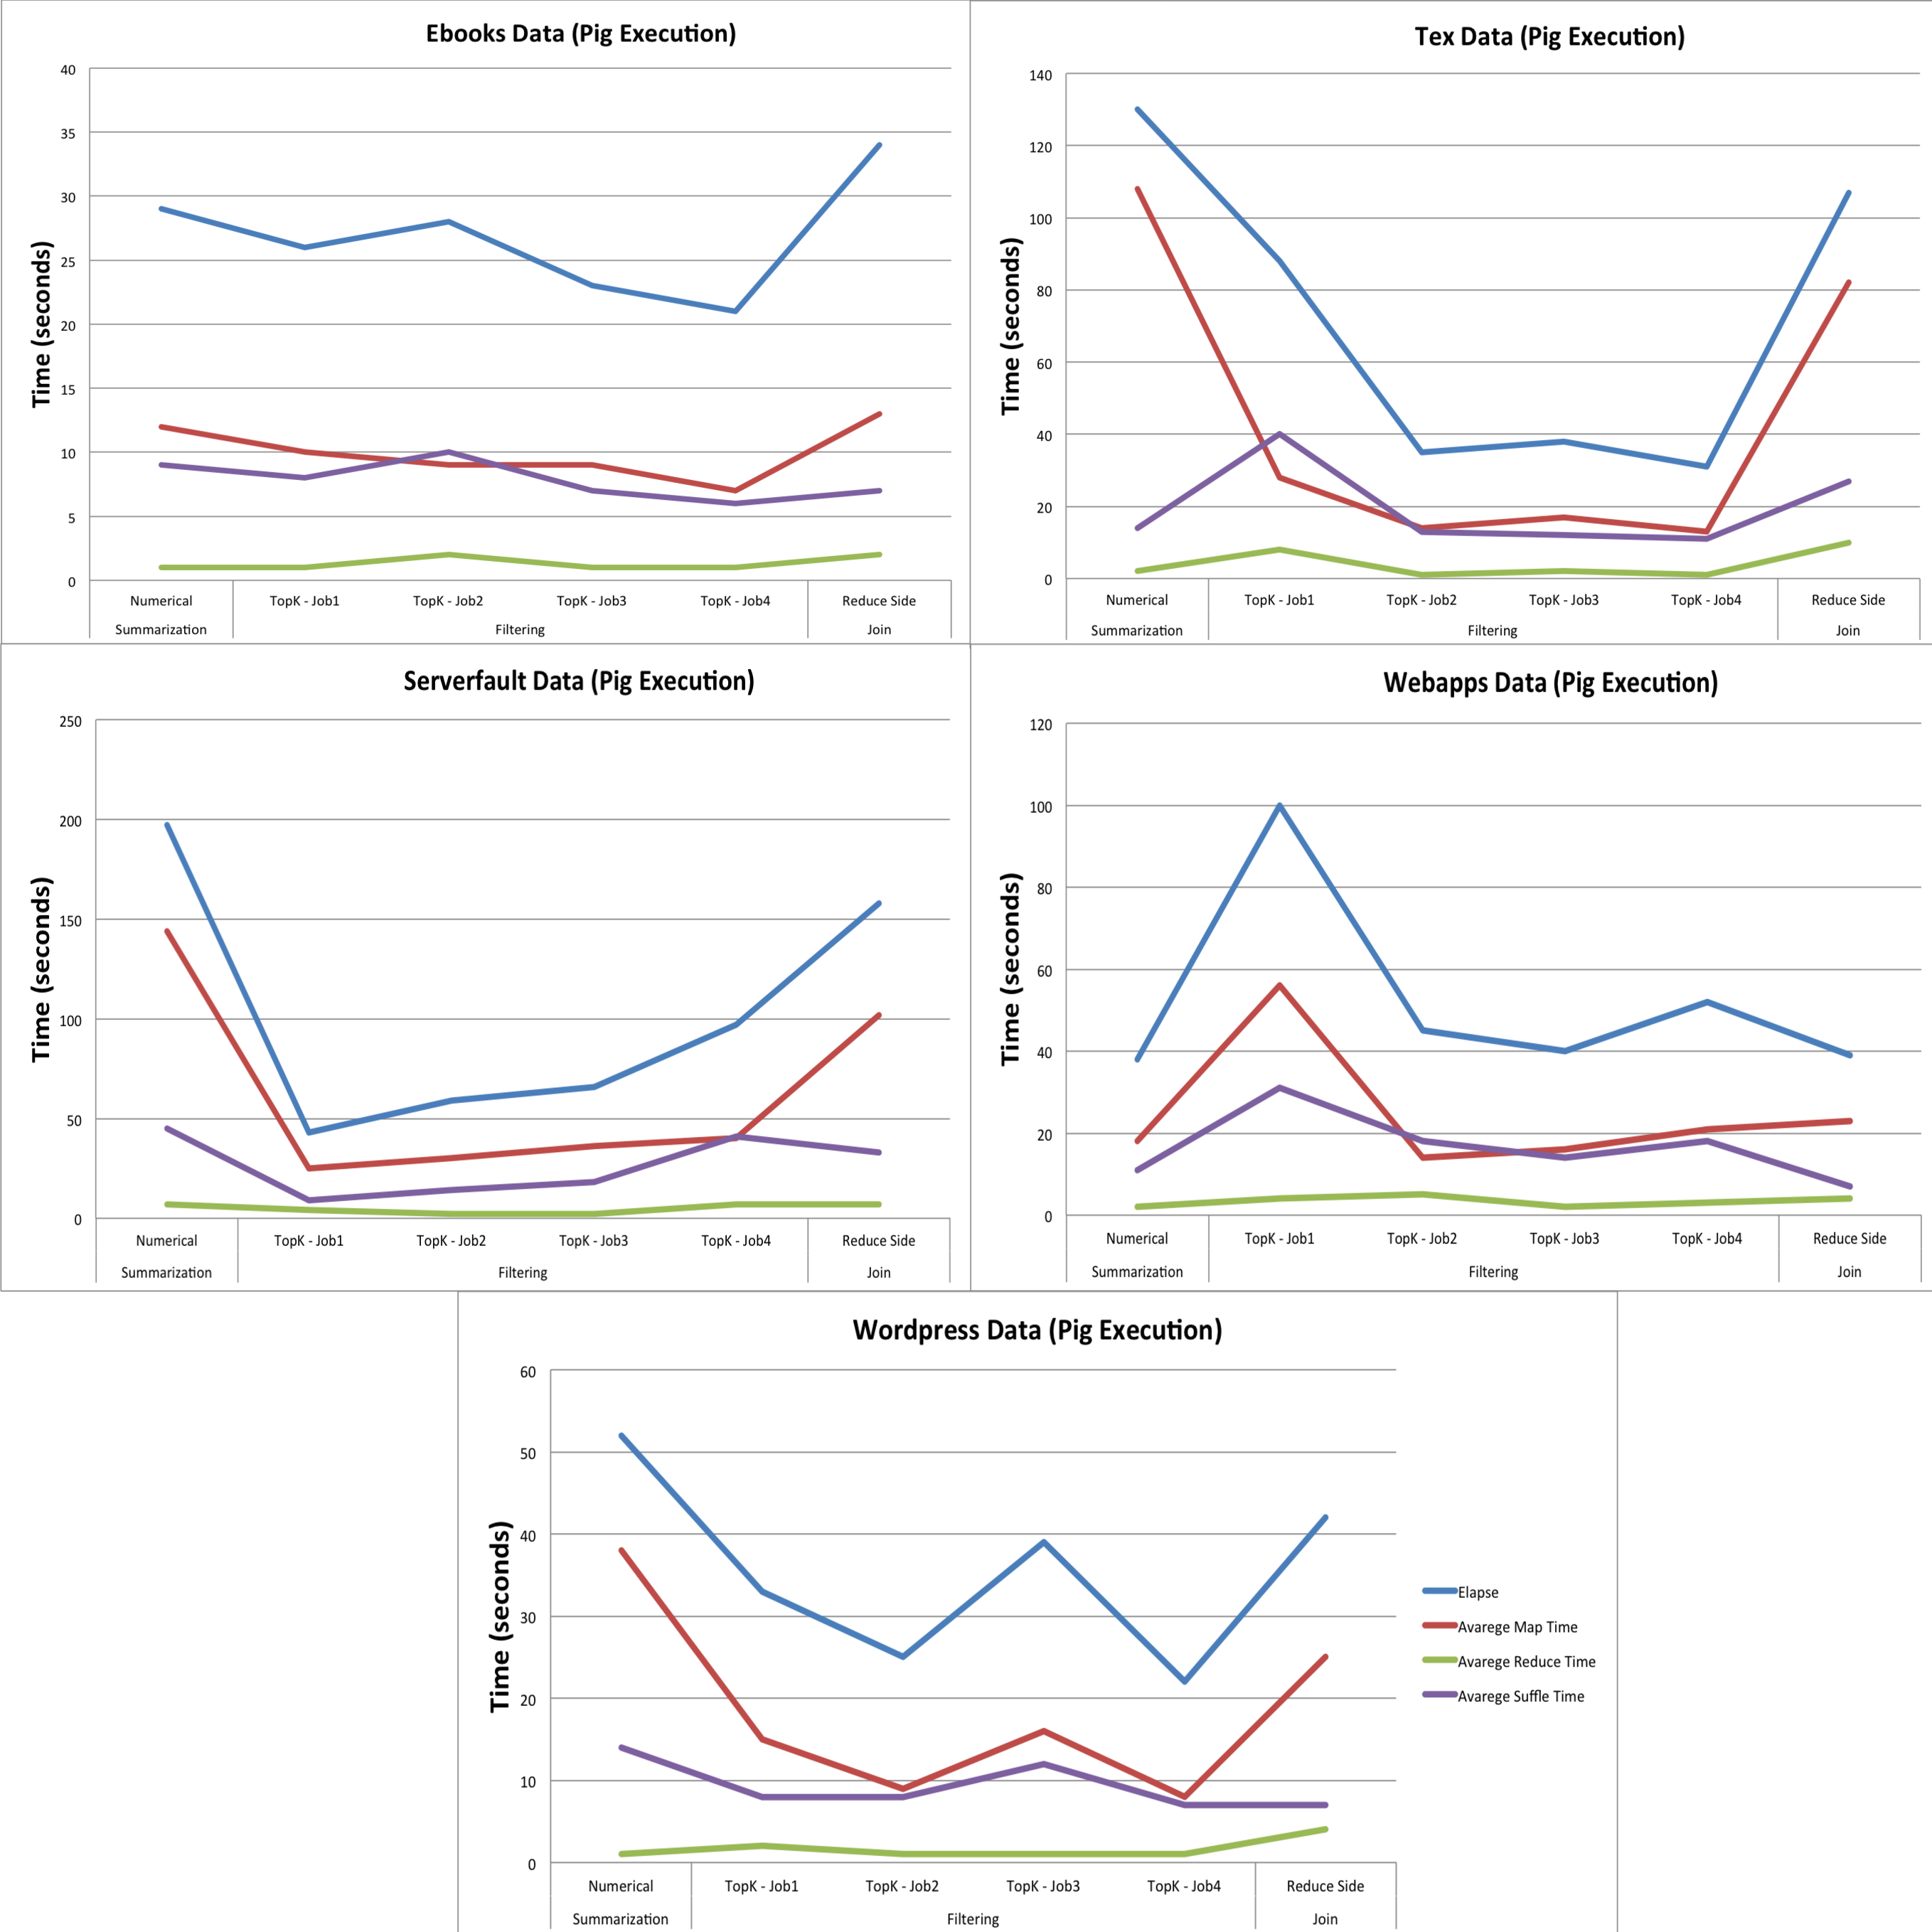
\includegraphics[width=0.99\textwidth]{figs/analysis-charts/compilation/pig.pdf}
% \caption{Pig Execution Data}
% \label{fig:patterns-domain}
% \end{figure} 
% 
% \begin{figure}[hbtp]
% \centering
% 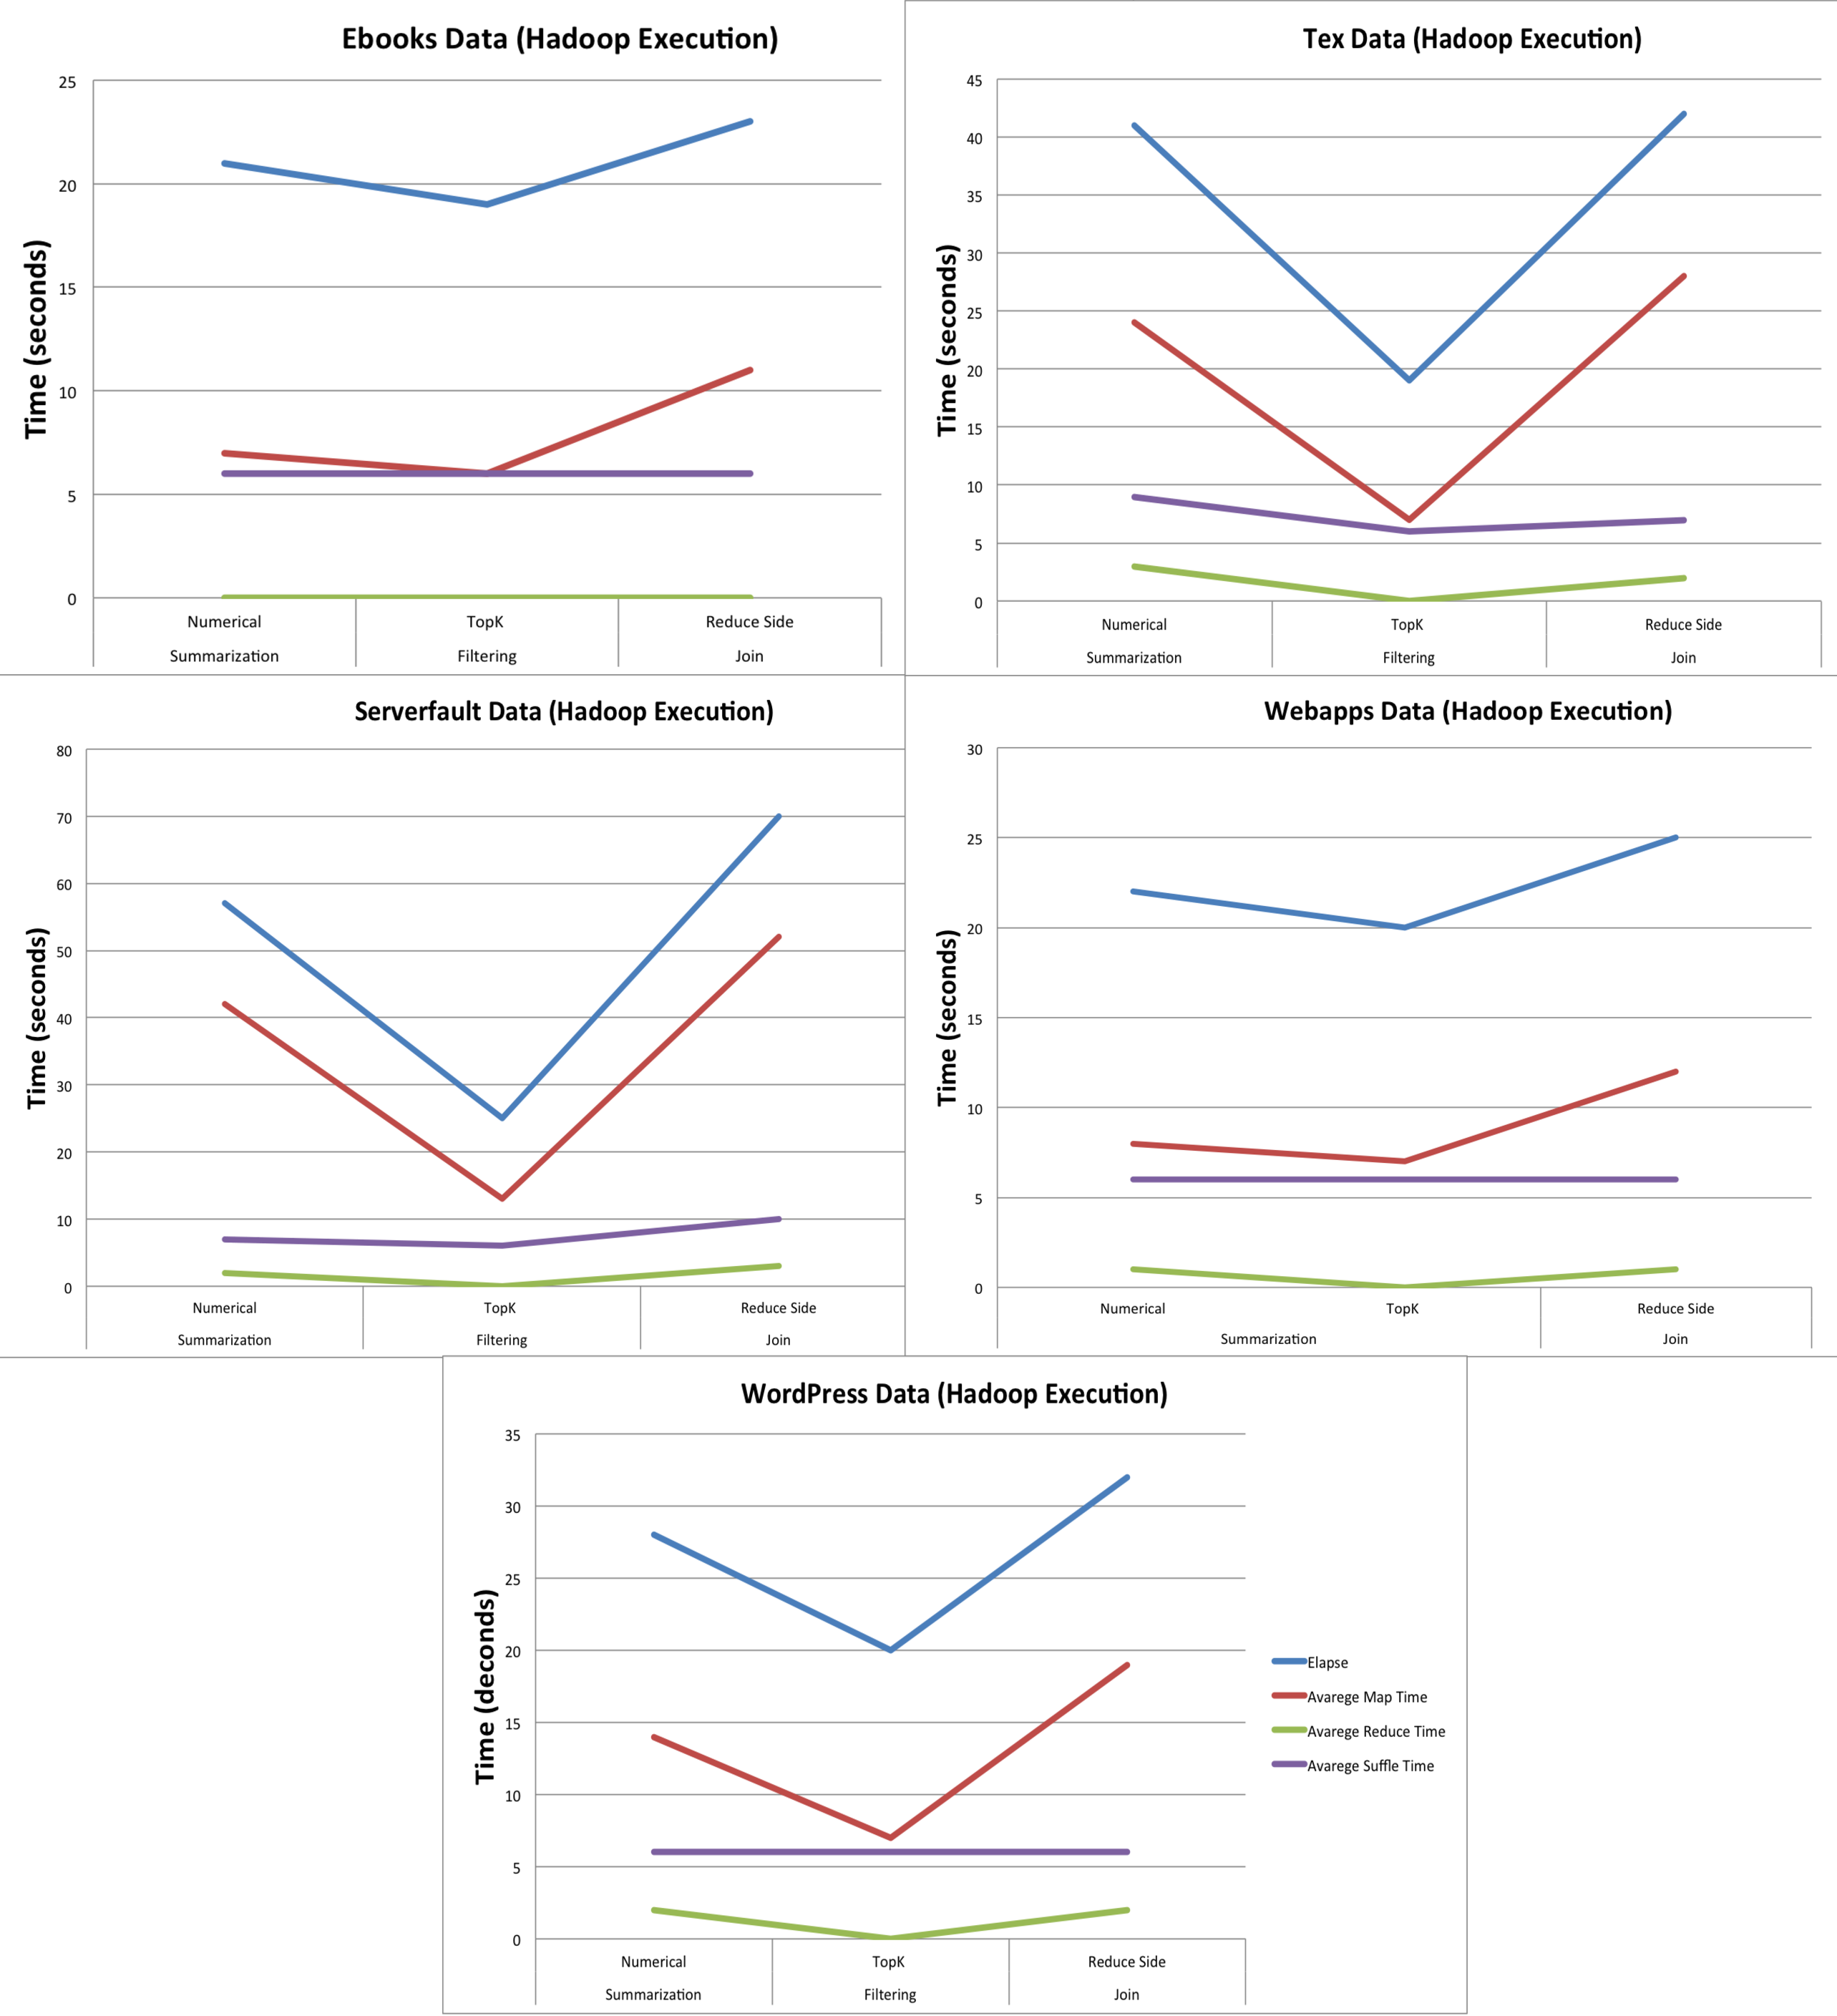
\includegraphics[width=0.99\textwidth]{figs/analysis-charts/compilation/hadoop.pdf}
% \caption{Hadoop Execution Data}
% \label{fig:patterns-domain}
% \end{figure}
% 
% \begin{figure}[hbtp]
% \centering
% 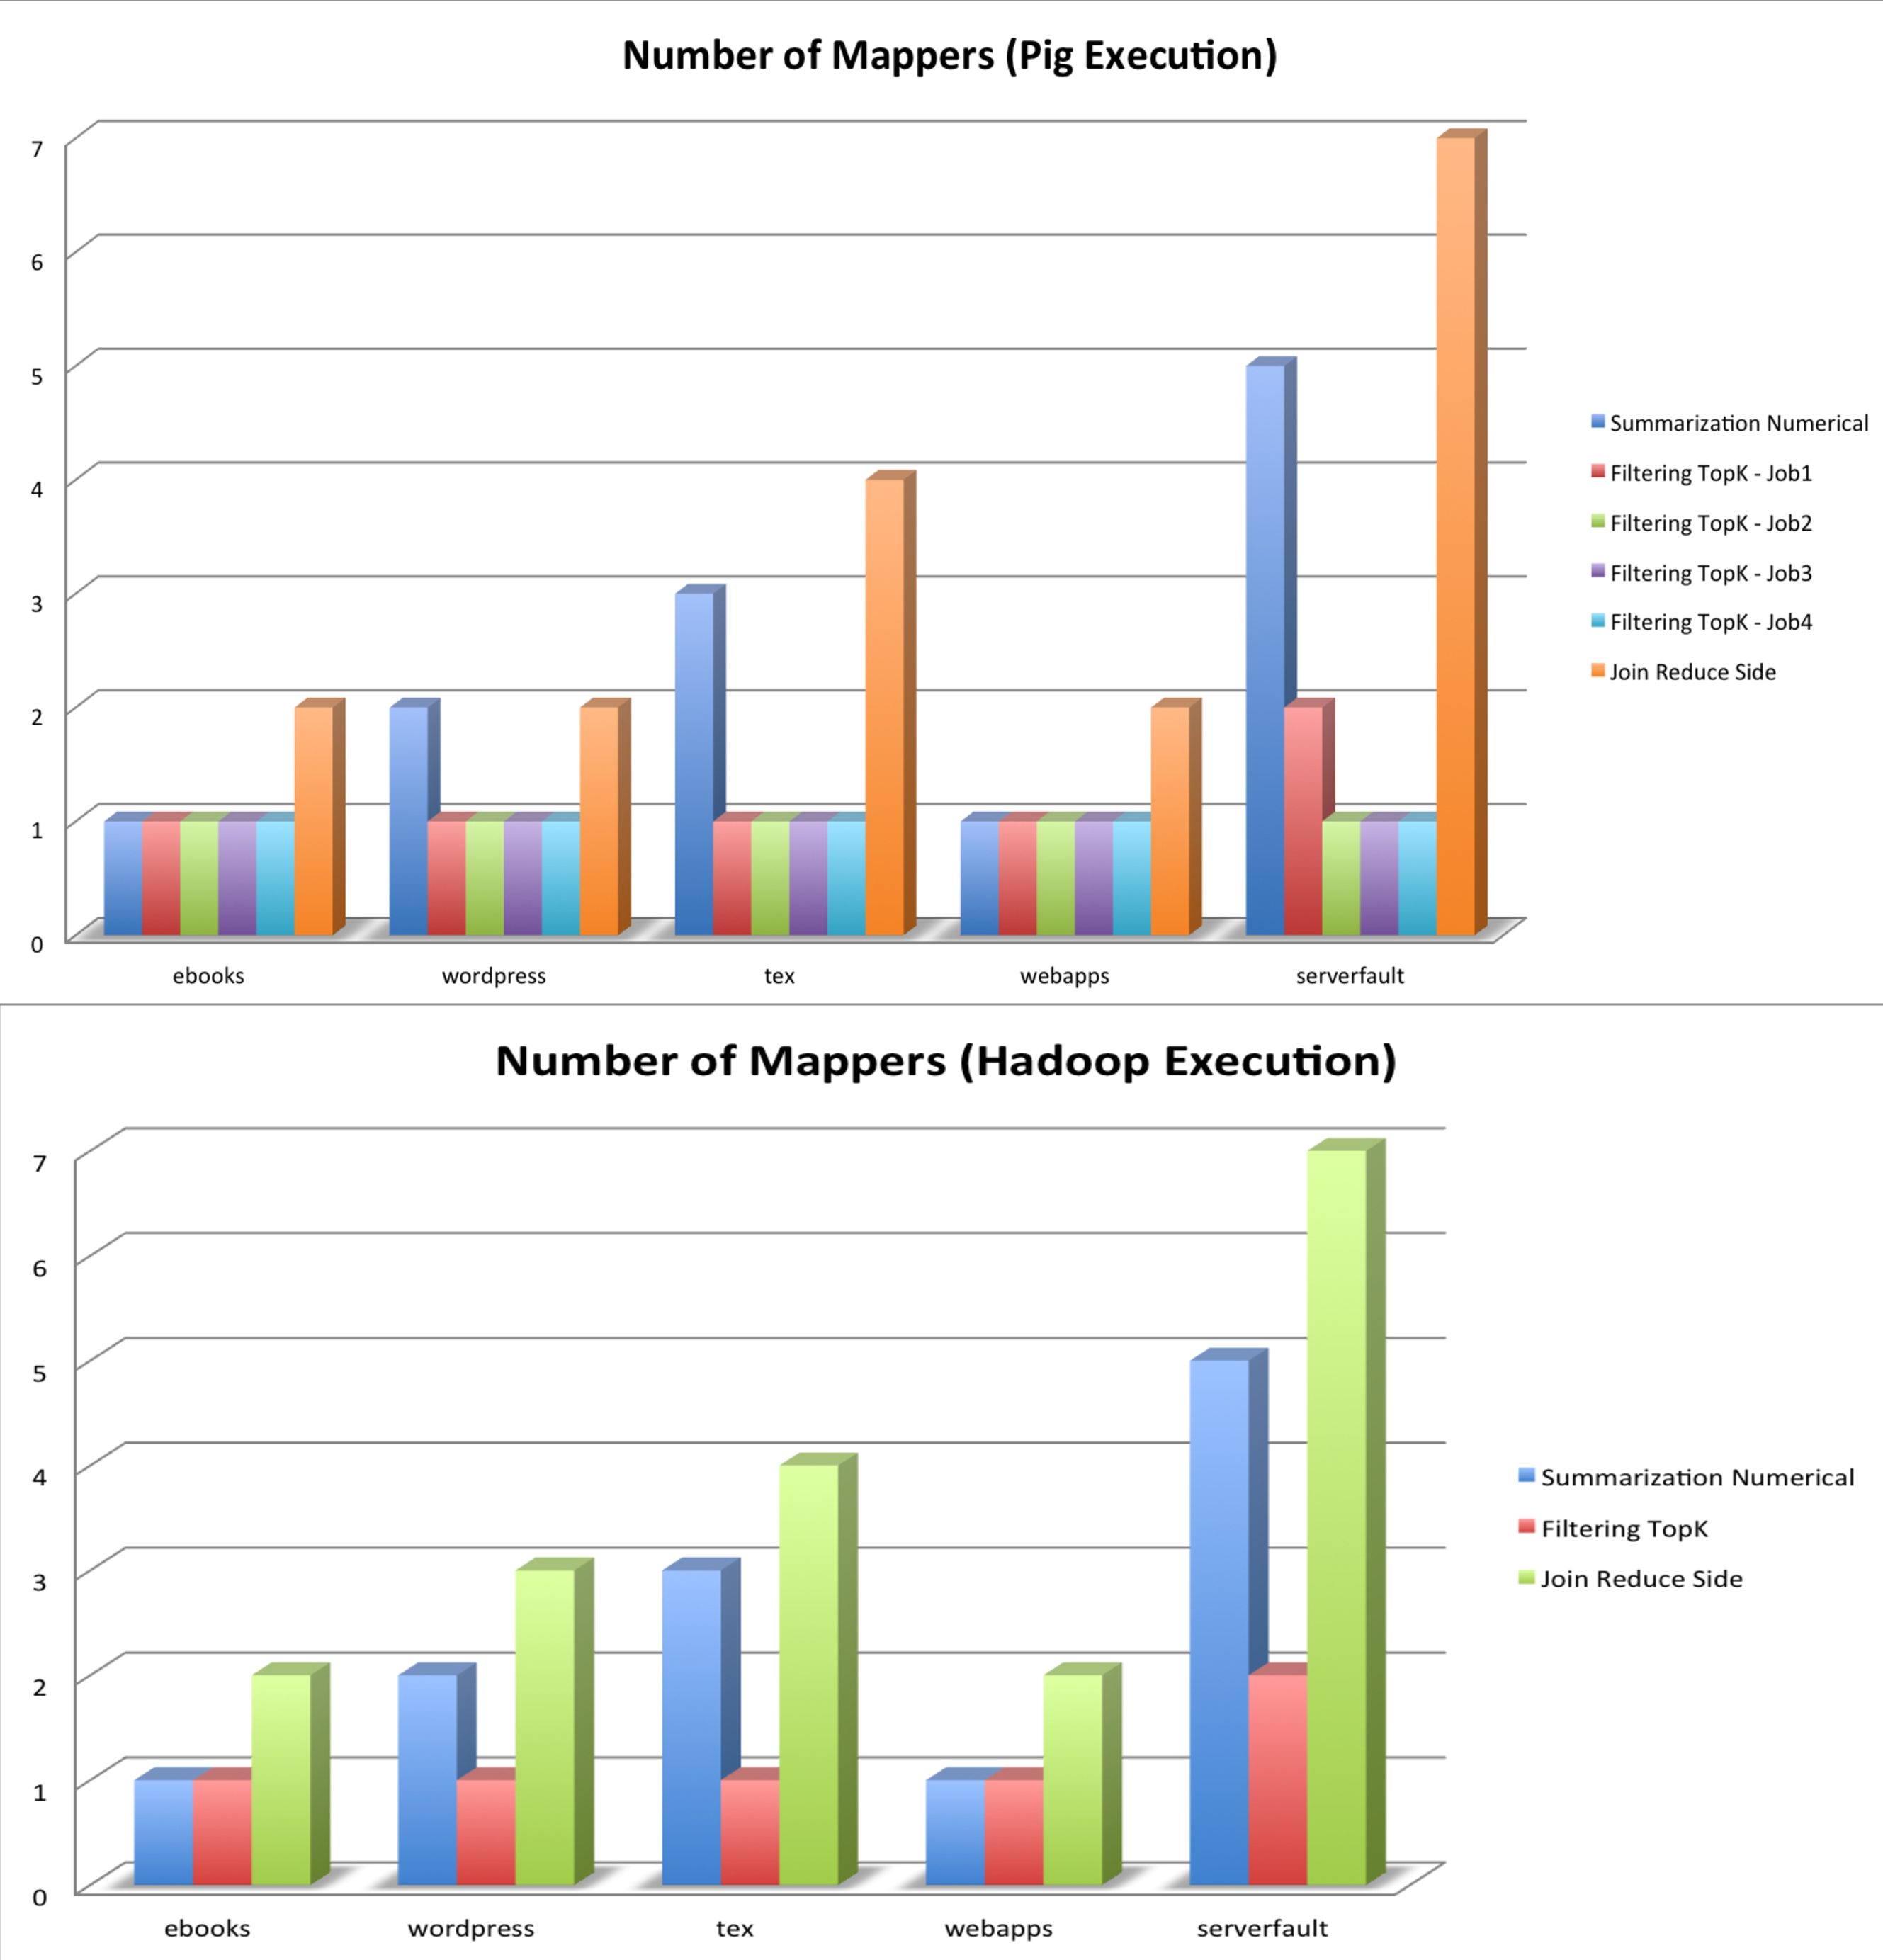
\includegraphics[width=0.99\textwidth]{figs/analysis-charts/compilation/mappers.pdf}
% \caption{Numbers of mappers criated during the execution}
% \label{fig:patterns-domain}
% \end{figure}


